\begin{center}
    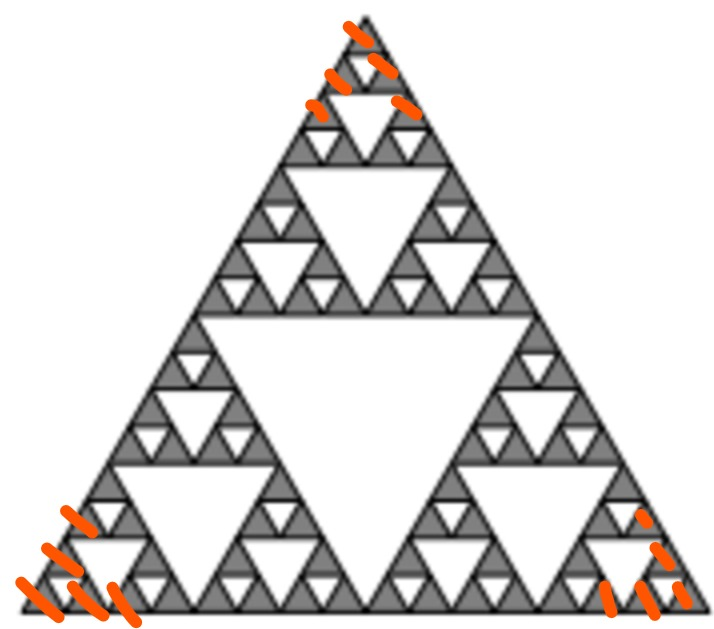
\includegraphics[scale=0.5]{solutions/section-5-0/diag-5-0-4.jpg}
\end{center}

This is one of the coverings of \(T_4\). The diameter is clearly \(\frac{13}{16}\) - as this is the distance between two opposite points in the figure. It also contains 66 out of 81 triangles - thus its value is \(\frac{\frac{13}{16}^s}{\frac{66}{81}}\) which is approximately \(0.8831093965\), notably less than \(0.9\). Hence \(a_4 \leq 0.8831093965 < 0.9\) so by theorem 5.0.2 the Hausdorff dimension is \(\leq 0.8831093965 < 0.9\), as required.